\documentclass{article}
\usepackage{graphicx} % Required for inserting images
\usepackage{wrapfig}

\usepackage{amsmath}
\usepackage{amssymb} % o amsfonts
\usepackage{braket}
\usepackage{float} 

\title{Appunti Quantum}
\author{Giuseppe Scordo}
\date{September 2025}

\begin{document}

\maketitle
I seguenti appunti fanno riferimento alle \textbf{Lecture Notes} di Scott Aaronson: \textit{Introduction to Quantum Information Science}, in cui vengono trattati temi relativi alla teoria dell'informazione, della computazione e della programmazione quantistica.

\section{Introduzione e Tesi di Turing-Church estesa}
L'informazione quantistica è una scienza interdisciplinare che attinge sia da fisica, matematica, informatica, ingegneria e addirittura filosofia.
\\Non si tratta solo di realizzare algoritmi utili, ma soprattutto capire come utilizzare la meccanica quantistica e saperla sfruttare. Prima di analizzare il tali meccanismi evidenziamo alcuni aspetti classici.
\begin{itemize}
    \item \textbf{Probabilità}: $(P\in [0,1])$   è il modo di indicare l'incertezza su eventi. Segue certi assiomi:
    \begin{itemize}
        \item Dato un set di $n$ eventi esaustivi e mutuamenti esclusivi la somma delle loro probabilità è $P_1 + P_2+\dots+P_n = 1$
        \item La probabilità di ogni evento soddisfa $P_i\ge0$
    \end{itemize}
Esiste l'opinione secondo cui, se sapessimo tutto sull'universo, come ad esempio la posizione e la velocità di ogni cosa, allora sarebbe possibile avere certezza sull'esito di ogni evento semplicemente calcolando.
    \medskip
    \\
    Immaginiamo di lanciare delle palline contro un muro in cui è presente un buco. È ovvio che aprendo nuovi fori nel muro allora la probabilità di passare dall'altra parte aumenta o al limite rimane uguale. Questa proprietà è detta \textbf{Monotonia}

    \item \textbf{Località}:  è l'idea che le cose si propaghino nell'universo ad una certa velocità. Una porzione di spazio interagisce solo con un'area ristretta attorno ad esso. In fisica questo principio emerge con la \textbf{Teoria della relatività ristretta}, che implica l'impossibilità di un segnale qualsiasi di propagarsi più velocemente della luce; ciò implicherebbe andare indietro nel tempo dal punto di vista dell'osservatore.
    \medskip
    \\
    In particolare il \textbf{Realismo Locale} è il principio secondo il quale la conoscenza istantanea di un informazione relativa ad un evento lontano può essere spiagata con la correlazione di variabili aleatorie.
    \\Ad esempio, se con un tuo amico sottoscrivete lo stesso abbonamento ad un giornale, ogni mattina alla consegna avrai la conoscenza di quale sia il titolo anche del suo giornale.
    \\La misura dello spin di due particelle in entanglement, seppure distanti nello spazio, non sembra molto dissimile dall'esempio del giornale, tuttavia come vedremo dopo non è compatibile con il realismo locale e con la teoria delle variabili casuali.

    \item \textbf{Tesi di Church Turing}: questa tesi afferma che ogni processo fisico può essere simulato da una macchina di Turing con qualsiasi precisione desiderata. 
    \\La \textbf{Tesi estesa di Church Turing} espande questo concetto affermando che quando simuliamo la realtà su un pc digitale vi è al massimo una crescita polinomiale in tempo, spazio, o ulteriori risorse.
    \medskip
    \\
    Applicando la meccanica quantistica a questi enunciati otteniamo alcune considerazioni:
    \begin{itemize}
        \item Il modo di calcolare le probabilità cambia violando l'assioma di monotonicità, cioè aumentando il numero di modi in cui un evento può accadere le sue probabilità possono diminuire
        \item Il principio di località permane ma quello di realismo locale viene rovesciato. Nella meccanica quantistica risulta ancora più evidente la differenza tra i due
        \item La tesi di Church Turing è in accordo con la meccanica quantistica mentre la tesi estesa sembrerebbe essere falsa poichè l'informatica quantistica ne costituisce un controesempio (Simulare un pc quantistico su uno classico prende risorse esponenziali). Tuttavia non è detto che non possa essere riformulata usando quest'ultima rendendo la macchina quantistica il vero modello universale.
    \end{itemize}
    \end{itemize}
    \section{Teoria della probabilità e Meccanica Quantistica}
    Il famoso fisico teorico Richard Feynman disse che tutto ciò che riguarda la meccanica quantistica può essere incapsulato nell'\textbf{Esperimento della Doppia Fenditura}.
    \\Questo famoso esperimento consiste nello "\textit{Sparare}" fotoni attraverso una fenditura, e successivamente attraverso due, per dimostrare la doppia natura della luce, sia come onda che come particella.
    \begin{figure}[h]
        \centering
        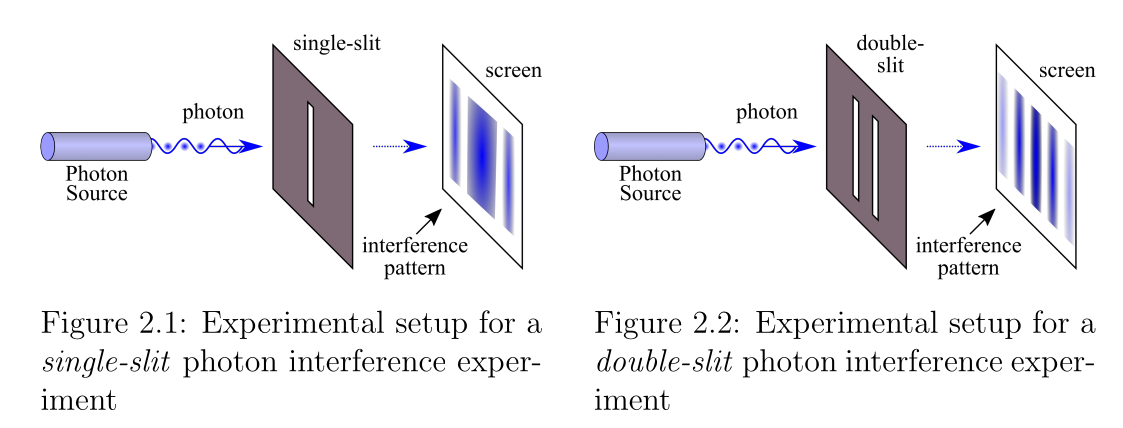
\includegraphics[width=1\linewidth]{Fenditure.png}
        \label{fig:fenditure}
    \end{figure}
    Alcune aree sullo schermo d'arrivo saranno più probabili, mentre altre lo saranno di meno. Potremmo spiegare ciò teorizzando che ogni fotone abbia ulteriori gradi di libertà che non conosciamo. Ma la cosa veramente strana è la seguente. Per alcuni intervalli sul seondo muro:
    \begin{itemize}
        \item Sia $P$ la probabilità che il fotone cada nell'intervallo con entrambe le fenditure aperte
        \item Sia $P_1$ la probabilità che cada nell'intervallo se solo una fenditura è aperta
        \item Sia $P_1$ la probabilità che cada nell'intervallo se solo la fenditura uno è aperta
        \item Sia $P_2$ la probabilità che cada nell'intervallo se solo la fenditura due è aperta
    \end{itemize}
    Potremmo pensare che $P = P_1 + P_2$ ma sperimentalmente ciò non avviene. Anche le aree che non vengono colpite quando entrambe le fenditure sono aperte possono essere colpite quando una sola è aperta.
    \\Potremmo pensare di osservare attraverso quale fenditura passi il fotone, ma facendo ciò lo stato finale cambia e ci ritroviamo davanti a qualcosa di più sensato, cioè semplicemente due fasce in cui la probabilità è masisma. Questa regressione alla probabilità classica dovuta all'interazione con l'ambiente è detta \textbf{Decoerenza}. Il bisogno di tenere le particelle isolate per evitare la decoerenza è la ragione per cui è così difficile costruire computer quantistici.
    \medskip
    \\
    \begin{figure}[ht]
        \centering
        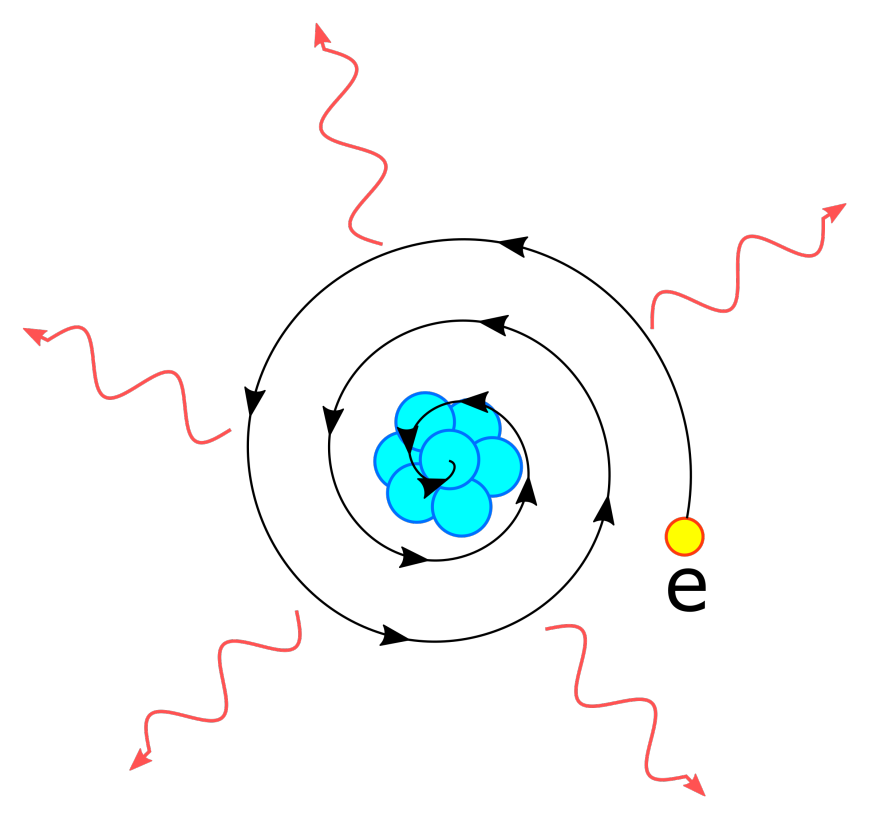
\includegraphics[width=0.5\linewidth]{energiaatomo.png}
        \label{fig:placeholder}
    \end{figure}
    La storia della fisica tra il 1900 e il 1926 consiste in una serie di scoperte che non corrispondono con le normali leggi della meccanica e della probabilità, a cui i fisici davano soluzioni complicate e disconnesse tra loro.
    \\Questo avvenne fino a quando Heisemberg, Schrodïnger etc... non elaborarono le leggi generali della meccanica quantistica.
    \\Brevemente, secondo il modello dell'atomo in cui l'elettrone ruota attorno al nucleo, l'elettrone dovrebbe perdere costantemente energia fino a scontrarsi con il nucleo.
    Per spiegare la stabilità dell'atomo i fisici allora hanno capito di dover cambiare il modo in cui calcoliamo le probabilità.
    \medskip
    \\
    Invece di definire la probabilità $P \in [0,1]$, si utilizzano \textbf{Ampiezze} $\alpha \in \mathbb{C}$. Le ampiezza possono essere sia positive che negative, o più in generale complesse. Il concetto fondamentale dietro le leggi della meccanica quantistica è che per descrivere un sistema isolato bisogna avere un'ampiezza per ogni possibile configurazione ottenuta misurandolo.
    \medskip
    \\
    La \textbf{Regola di Born} dice che la probabilità di osservare un particolare risultato è data dal quadrato del valore assoluto dell'ampiezza:
    \begin{equation}
        P = |\alpha|^2= \text{Re}(\alpha)^2+\text{Im}(\alpha^2)
    \end{equation}
    Rivediamo l'esperimento della doppia fenditura utilizzando le ampiezze:
    \begin{itemize}
        \item Sia $\alpha$ l'ampiezza totale di avere una certa posizione sullo schermo.
        \item Sia $\alpha_1$ l'ampiezza associata di avere una certa posizione sullo schermo con la fenditura uno aperta
        \item Sia $\alpha_2$ l'ampiezza associata di avere una certa posizione sullo schermo con la fenditura due aperta
    \end{itemize}
    Allora analogamente al caso classico avremmo:
    $$\alpha = \alpha_1+\alpha_2$$
    Ma la probabilità di vedere quello stato diventa:
    $$P = |\alpha|^2 = |\alpha_1 + \alpha_2|^2 = |\alpha_1|^2 + |\alpha_2|^2 + \alpha^*_1\alpha_2 + \alpha_1\alpha^*_2$$
    Se per esempio $\alpha_1 = 1/2$ e $\alpha_2 = -1/2$ allora $P = 0$ se entrambe le fenditure sono aperte, mentre $P = 1/4$ se una sola è aperta. Questo fenomeno è detto \textbf{Interferenza}. Quindi la stabilità dell'elettrone è dovuta al fatto che ci sono molte strade che l'elettrone può percorrere, alcune con ampiezza positiva ed altre con ampiezza negativa che si cancellano a vicenda.
    \subsection{Approccio con l'algebra lineare alla teoria della probabilità}
    Usiamo l'algebra lineare per modellare gli stati del sistema come vettori e le sue trasformazioni come trasformazioni lineari. Scritto formalmente:
    \begin{equation}
        M \begin{bmatrix}
            a_1
            \\a_2
        \end{bmatrix}
        = 
        \begin{bmatrix}
            a_1'
            \\a_2'
        \end{bmatrix}
    \end{equation}
    Per il momento concentriamoci sulla probabilità classica. Pensiamo al lancio di una moneta in cui $p = P(\text{testa})$ e $q = P(\text{croce})$.

    $$
        \begin{bmatrix}
            p \\ q
        \end{bmatrix}
        \hspace{0.2cm}
        p,q \ge0 , \hspace{0.2cm}
        p+q = 1
    $$
    Possiamo applicare la trasformazione \textit{gira la moneta al contrario}:
    $$
        \begin{bmatrix}
            0 & 1 \\ 1 & 0 
        \end{bmatrix}
        \begin{bmatrix}
            p \\ q
        \end{bmatrix}
        = 
        \begin{bmatrix}
            q \\ p
        \end{bmatrix}
    $$
    In questo caso vuol dire che le probabilità sono state invertite, visto che se prima era testa ora è croce e così via.
    \\Possiamo definire il lancio equo come segue
    $$
        \begin{bmatrix}
            \frac{1}{2} & \frac{1}{2}
            \\ \frac{1}{2} & \frac{1}{2} 
        \end{bmatrix}
        \begin{bmatrix}
            p \\ q
        \end{bmatrix}
        = 
        \begin{bmatrix}
            \frac{1}{2}
            \\\frac{1}{2}
        \end{bmatrix}
    $$
    Possiamo cambiare ancora le regole dicendo che se abbiamo testa lanciamo di nuovo la moneta, ma se abbiamo croce la cambiamo in testa.
    $$
        \begin{bmatrix}
            \frac{1}{2} & 1
            \\ \frac{1}{2} & 0 
        \end{bmatrix}
        \begin{bmatrix}
            p \\ q
        \end{bmatrix}
        = 
        \begin{bmatrix}
            q+\frac{p}{2}
            \\\frac{p}{2}
        \end{bmatrix}
    $$
    Possiamo vederla come:
    \begin{itemize}
        \item $P(\text{testa}| \text{testa}) = \frac{1}{2}$ se esce testa la rilanciamo
        \item $P(\text{testa}| \text{croce}) = 1$ se esce croce giriamo la moneta
        \item $P(\text{croce}| \text{testa}) = \frac{1}{2}$ se esce testa la rilanciamo
        \item $P(\text{croce}| \text{croce}) = 0$ se esce croce giriamo la moneta
    \end{itemize}
    Quali matrici possiamo utilizzare come trasformazioni nel lancio di moneta?
    \\Prima di tutto sappiamo che ogni elemento deve essere non negativo, poichè la probabilità classica non ne contempla la possibilità, e inoltre la somma di ogni colonna deve essere uno, per calcolare le probabilità totali. Una matrice che possiede queste proprietà è detta \textbf{Matrice stocastica}.
    \medskip
    \\
    Adesso pensiamo al flip di due bit. $a =P(0)$ e $b =P(1)$ per il primo, $c =P(0)$ e $d =P(1)$ per il secondo. 
    $$
    \begin{array}{c}
         0 \\
         1 
    \end{array}
    \begin{bmatrix}
        a \\
        b
    \end{bmatrix}
    \hspace{0.5cm}
    \begin{array}{c}
         0 \\
         1 
    \end{array}
    \begin{bmatrix}
        c \\
        d
    \end{bmatrix}
    $$
    Per definire un unico stato del sistema combinando entrambi utilizziamo il \textbf{Prodotto Tensoriale}:
    $$
    \begin{bmatrix}
        a \\ b
    \end{bmatrix}
    \otimes
    \begin{bmatrix}
        c \\ d
    \end{bmatrix}
    = 
    \begin{bmatrix}
        ac \\ ad \\ bc \\bd
    \end{bmatrix}
    $$
    Notiamo che non tutti i vettori derivano dal prodotto tensoriale, ad esempio:
    $$
        \begin{bmatrix}
        ac \\ ad \\ bc \\bd
    \end{bmatrix}
    =\begin{bmatrix}
        \frac{1}{2} \\ 0 \\ 0 \\ \frac{1}{2}
    \end{bmatrix}
    $$
    Che non può essere scritto come prodotto tensoriale di due vettori.
    \medskip
    \\
    Anche in questo caso possiamo usare matrici stocastiche per descrivere trasformazioni, ad esempio l'operazione \textbf{CNOT} flippa il seconda qubit se il primo ha valore 1. È una delle matrici più utilizzate nel calcolo quantistico.
    $$
        \textbf{CNOT} = 
    \begin{bmatrix}
        1 &0 &0 &0 \\ 0 &1 &0 &0\\ 0 & 0& 0&1\\ 0&0&1&0
    \end{bmatrix}
    $$
    Applicandola al vettore definito prima otteniamo una configurazione in cui se il primo qubit è 1, il secondo sarà sempre zero:
    $$
        \begin{bmatrix}
        1 &0 &0 &0 \\ 0 &1 &0 &0\\ 0 & 0& 0&1\\ 0&0&1&0
    \end{bmatrix}
    \begin{bmatrix}
        \frac{1}{2} \\ 0 \\ 0 \\ \frac{1}{2}
    \end{bmatrix}
    =
    \begin{bmatrix}
        \frac{1}{2} \\ 0 \\ \frac{1}{2} \\ 0
    \end{bmatrix}
    $$
    La configurazione che abbiamo raggiunto non è esprimibile anch'essa come prodotto tensoriale, e si dice \textbf{Correlata}. L'operazione CNOT quindi è utile per creare correlazione nelle distribuzioni.
    \medskip
    \\
    La meccanica quantistica sostanzialmente segue questo processo di modellazione con la differenza dell'uso delle ampiezze. Possiamo rappresentare una trasformazione in meccanica quantistica utilizzando matrici di stato.
    $$
        \begin{bmatrix}
            \\&U&\\
            \
        \end{bmatrix}
        \begin{bmatrix}
            a_1 \\a_2 \\ a_3 
        \end{bmatrix}
        = \begin{bmatrix}
            b_1 \\ b_2 \\ b_3
        \end{bmatrix}
    $$
    In cui viene preservata la somma dei quadrati $\sum^3_i |a_i|^2 = \sum^3_i |b_i|^2 = 1$ che per la regola di Born indica che la probabilità totale è sempre uno. Queste matrici sono dette \textbf{Matrici unitarie} e godono di numerose proprietà fondamentali in meccanica quantistica.

    \section{Regole basi della meccanica quantistica}
    \subsection{Stati quantistici e notazione Ket}
    Uno stato quantistico (tecnicamente uno \textit{stato puro}) è un vettore in $\mathbb{C}^N$ che descrive lo stato del sistema quantistico a $N$ dimensioni.
    \\Il \textbf{Qubit} è il più semplice tra i sistemi quantistici. È un sistema a due livelli in cui le ampiezze  sono associate a 0 e 1.
    \\Utilizzando la notazione introdotta da Paul Dirac possiamo scrivere i vettori degli stati quantistici in \textbf{Ket Notation}
    $$
        \begin{bmatrix}
            \alpha \\ \beta
        \end{bmatrix}
        = \alpha \ket{0} + \beta \ket{1}
    $$
    Dove $\ket{0} = \begin{bmatrix} 1\\0\end{bmatrix}$ e $\ket{1} = \begin{bmatrix} 0\\1\end{bmatrix}$. Inoltre utilizziamo $\ket{\psi}$ per riferirci ad un generico stato quantistico. La notazione Ket semplifica notevolmente i calcoli evidenziando solo i valori che ci interessano.
    \\Spesso ci troveremo a dover utlizzare anche la trasposta coniugata, ad esempio per calcolare la norma del vettore
    $$||v||^2 = \begin{bmatrix}
        \alpha^* & \beta^*
    \end{bmatrix}
    \hspace{0.1cm}
    \begin{bmatrix}
        \alpha \\ \beta
    \end{bmatrix}
    = |\alpha|^2 + |\beta|^2 
    $$
    Il coniugato trasposto di uno stato \textbf{Ket} $\ket{\psi} = \alpha\ket{0}+\beta\ket{0}$ si chiama \textbf{Bra} $\bra{\psi} = \alpha^*\bra{0}+\beta^*\bra{1}$, che possiamo utilizzare per esprimere il prodotto interno tra due stati $\ket{x}$ e $\ket{y}$ come $\braket{x|y}$. La norma del vettore $\ket{\psi}$ in questa notazione è
    $||\psi|| = \braket{\psi|\psi}$. Il prodoto interno per come è definito gode della seguente proprietà $\braket{x|y} = \braket{{y|x}}^*$. Per la coniugata trasposta utilizzeremo il simbolo \textit{dagger} $\dagger$.
    \\
    L'insieme dei possibili stati puri a coefficienti reali di un qubit definisce una circonferenza. Gli stati puri a coefficienti complessi invece definiscono una sfera, detta \textbf{Sfera di Bloch}, che approfondiremo successivamente. Oltre agli stati $\ket{0}$ e $\ket{1}$ introduciamo altri quattro stati che incontriamo molto frequentemente.

    \begin{figure}[H]
        \centering
        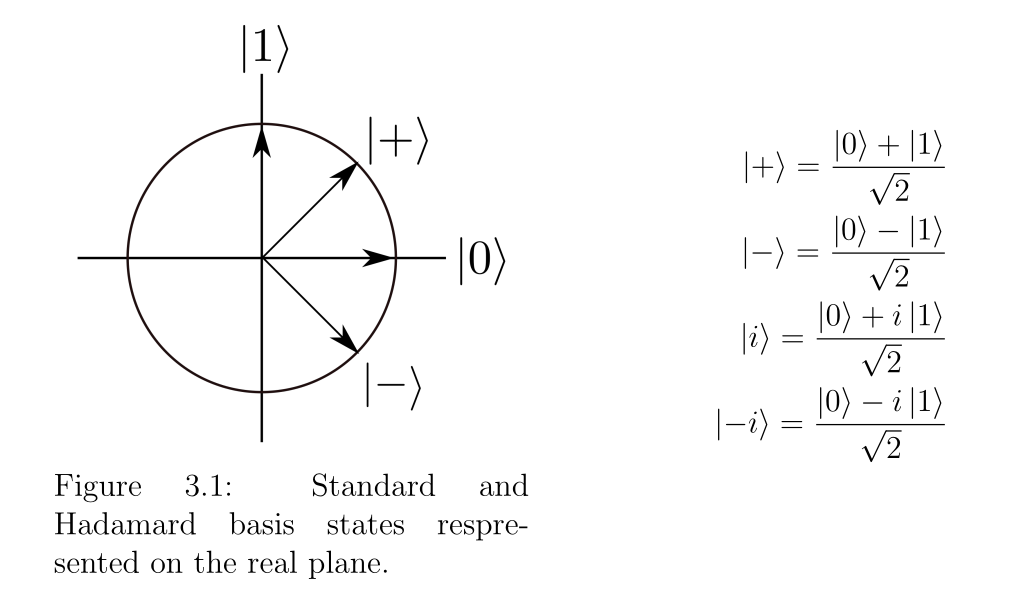
\includegraphics[width=1\linewidth]{Circonferenza.png}
        \label{fig:placeholder}
    \end{figure}
    La coppia $\{\ket{+},\ket{-}\}$ è detta \textit{Base di Hadamard}. La figura mostra gli stati della base di Hadamard sul piano reale.

    \subsection{Trasformare stati quantistici}
    Così come per la probabilità classica possiamo modificare lostato quantistico attraverso trasformazioni lineari
    \begin{equation}
    U\ket{\psi} = U \begin{bmatrix}
        \alpha \\ \beta
    \end{bmatrix} 
    = \begin{bmatrix}
        \alpha'\\\beta'
    \end{bmatrix}
    \end{equation}
    Una condizione per la validità della trasformazione negli stati quantistici è che questa sia \textbf{unitaria}, cioè: Una trasformazione $U$ è unitaria se $|\alpha|^2+|\beta|^2 = |\alpha'|^2 + |\beta'|^2$ per ogni vettore in input. In parola povere se preserva la norma del vettore.
    
    \subsubsection{Esempi di trasformazioni unitarie su un Qubit}
    \[
    \begin{array}{cccc}
    % Prima riga: Le matrici
    \begin{bmatrix} 1 & 0 \\ 0 & 1 \end{bmatrix} &
    \begin{bmatrix} 0 & 1 \\ 1 & 0 \end{bmatrix} &
    \begin{bmatrix} 1 & 0 \\ 0 & i \end{bmatrix} &
    \begin{bmatrix} \cos(\theta) & -\sin(\theta) \\ \sin(\theta) & \cos(\theta) \end{bmatrix} \\[-1ex]
    \\
    % Seconda riga: Le definizioni
    \text{Identity} & \text{NOT Gate} & \text{Relative Phase Shift} & \text{2D-Rotations}
    \end{array}
    \]
    La terza matrice in particolare mappa $\ket{0}\rightarrow \ket{0}$ e $\ket{1}\rightarrow i\ket{1}$; possiamo di fatto rimpiazzare $i$ nella matrice con la forma esponenziale complessa $e^{i\theta}$, dall'equazione di Eulero
    \begin{equation}
        e^{i\theta} = \cos(\theta) + i \sin(\theta)
    \end{equation}
    Anche le rotazioni preservano la norma; possiamo usare l'ultima matrice per ruotare lo stato nel piano reale di un angolo $\theta$. Denotiamo questa famiglia di matrici con $R_\theta$.
    \\
    Visto che una matrice unitaria,$U$, preserva la norma di un vettore segue che ne preserva anche il prodotto interno $\braket{\psi|\psi}$. Questo implica una serie di uguaglianze
    \[
    \braket{\psi|\psi} = (\ket{\psi})^\dagger\ket{\psi} = (U\ket{\psi})^\dagger U\ket{\psi} = \bra{\psi}U^\dagger U \ket{\psi} 
    \]
    Questo è vero per ogni $\ket{\psi}$ se $U^\dagger U = I$; ciò implica che per una matrice unitaria $U^\dagger = U^{-1}$. Implica inoltre che le righe di $U$ devono formare una base ortonormale. Viceversa è chiaro che se $U^{-1} = U^\dagger$ la matrice è unitaria. Quindi per verificare se $U$ è unitaria possiamo controllare se $U^\dagger U= I$, o se le sue righe (o colonne) formano una base ortonormale.
    \medskip
    \\ Una \textbf{Matrice ortogonale} è sia unitaria che a valori reali. Ogni matrice ortogonale è prodotto di matrici di rotazione e riflessioni. Per esempio per la matrice $R_{\pi/4}$ applicata ripetutamente su $\ket{0}$ ottiene un giro completo dopo otto applicazioni.


    
    \subsection{Interferenza Quantistica}
    Nel modno classico, per un evento con più esiti che avvengono in maniera casuale, non importa in che maniera avvenga, nel complesso rimane un evento casuale.
    \\Nel mondo quantistico a volte possiamo però applicare una trasformazione unitaria ad uno stato in sovrapposizione ottenendo un risultato deterministico, anche se la risposta sarebbe stata casuale applicandola ad una singola componente dello stato. Molti di questi fenomeni possono essere spiegati in termini di \textbf{Interferenza quantistica}. Supponiamo per esempio di partire dallo stato $\ket{0}$. Applichiamo due volte la trasformazione unitaria che mappa $\ket{0}\rightarrow\ket{+}$ e $\ket{1}\rightarrow \ket{-}$. 
    \begin{figure}[H]
        \centering
        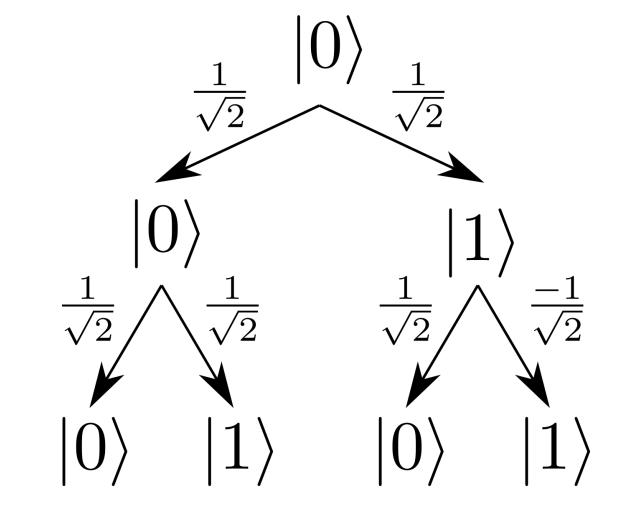
\includegraphics[width=0.5\linewidth]{Path.png}
        \label{fig:placeholder}
    \end{figure}
    Per ottenere l'ampiezza di probabilità associata ai possibili risultati facciamo il prodotto delle ampiezze nel percorso associato. Una volta ottenuta l'ampiezza per un particolare output facciamo la somma delle ampiezze ottenute per esso. In questo modo otteniamo che l'ampiezza per $\ket{0}$ è $1$ mentre per $\ket{1}$ è $0$. In pratica abbiamo un'interferenza costruttiva su $\ket{0}$ e un'interferenza distruttiva su $\ket{1}$
    \subsubsection{Fase Globale e Relativa}
    Essendo le trasformazioni unitarie, $U$, trasformazioni lineari, vale che $U (-\ket{0}) = -U\ket{0}$ o in generale
    $U (c\ket{\psi}) = cU\ket{\psi}$ per qualche costante $c$. Se $c$ è un numero complesso unitario ($e^{i\theta}$) diciamo che esso è una \textbf{Fase globale}. Lo stato $\ket{\psi}$ e $e^{i\theta}\ket{\psi}$ sono fisicamente indistinguibili, cioè la fase globale non può essere osservata. È come se stessimo semplicemente \textit{"spostando"} il sistema quantistico rispetto al sistema di riferimento.
    Tuttavia la \textbf{Fase Relativa} invece è osservabile! Per distinguere $\ket{+}$ da $\ket{-}$ basta applicare una rotazione di 45° ($R_{\pi/4}$) e misurare controllando se si ottiene $\ket{0}$ o $\ket{1}$. L'osservabilità delle fasi relative è douta proprio alla possibilità di applicare una sequenza di operazioni che ne determino il risultato; per le fasi globali non abbiamo procedure del genere. 


    \section{Gate Quantistici e Circuiti, Quantum Zeno e La Bomba di Elitzur-Vaidman}
    \subsection{Gate Quantistici}
    Nella teoria dell'informazione quantistica ci riferiamo spesso a piccole trasformazioni unitarie come \textbf{Gates}, a cui associamo nomi e simboli specifici. Ad esempio la matrice $\begin{bmatrix}
        0 & 1 \\1 & 0
    \end{bmatrix}$
    è la matrice NOT. Analogamente possiamo definire la matrice $\sqrt{\text{NOT}}$
    \begin{equation}
    \sqrt{\text{NOT}} = \frac{1}{2} \begin{bmatrix}
        1+i &1-i \\ 1-i & 1+i
    \end{bmatrix}
    \end{equation}
    Che ovviamente soddisfa la proprietà $\sqrt{\text{NOT}} \sqrt{\text{NOT}} = \text{NOT}$
    \medskip
    \\ Uno dei Gates più utilizzati è il cosiddetto \textbf{Hadamard Gate}
    \begin{equation}
        H = \frac{1}{\sqrt{2}}\begin{bmatrix}
            1 & 1\\ 1 & -1
        \end{bmatrix} 
    \end{equation}
    È il gate che ci permette di mapare la base computazionale $\{\ket{0},\ket{1}\}$ nella base di Hadamard $\{\ket{+},\ket{-}\}$ e viceversa.
    \medskip
    \\ \textit{Nota: formano due basi ortogonali con la proprietà specifica che avere massima certezza su $\{\ket{0},\ket{1}\}$ significa avere massima incertezza su $\{\ket{+},\ket{-}\}$ e viceversa}
    \medskip
    \\ Un altro esempio di gate per il cambiamento di base è
    \begin{equation}
    \frac{1}{\sqrt{2}}
    \begin{bmatrix}
        1 & 1 \\ i &-i
    \end{bmatrix}
    \end{equation}
    che mappa da $\{\ket{0},\ket{1}\}$ a $\{\ket{i},\ket{-i}\}$. Perchè vogliamo cambiare base? Negli algoritmi quantistici pensiamo agli stati come vettori, quindi scegliamo spesso la base più conveniente. I cambiamenti di base sono molto frequenti negli algoritmi quantistici.
    \subsubsection{Regola di Born Generalizzata}
    Misurando uno stato $\ket{\psi}$ nella base ortonormale $\{ \ket{V_0}, \dots, \ket{V_{N-1}} \}$, si ottiene lo sato $\ket{V_i}$ con probabilità $|\braket{V_i|\psi}|^2$. Quindi la probabilità di ottenere $\ket{V_i}$ è dato dal modulo quadro della proiezione su quel vattore della base. Per misurare su una base arbitraria possiamo applicare trasformazioni unitarie per cambiare base. Ad esempio possiamo applicare alla base precedente una trasformazione unitaria, $U$, tale che $U\ket{V_0} = \ket{0}$, $U\ket{V_1} = \ket{1} \dots$ e misurare nella base standard  $\{ \ket{0}, \dots, \ket{N-1} \}$
    \medskip
    \\ \textit{Nota: esiste una corrente di pensiero per cui le trasformazioni unitarie sono le uniche cose che esistono, mentre le misurazioni no. Esiste anche la visione diametralmente opposto, ma approfondiremo nella sezione sulle interpretazioni.}

    \subsection{Proprietà Generali dei Gate Quantistici e Misurazioni}
    Le trasformazioni unitarie sono:
    \begin{itemize}
        \item \textbf{Invertibili:} Poiché, per preservare la norma, $U^\dagger U = I$, il che implica $U^{-1} = U^\dagger$.
        \begin{itemize}
            \item In parole povere, la trasformazione $\ket{\psi} \to U\ket{\psi}$ può essere invertita applicando $U^\dagger$, poiché $U^\dagger U \ket{\psi} = I \ket{\psi} = \ket{\psi}$.
        \end{itemize}
        \item \textbf{Deterministiche:} Non c'è nulla di probabilistico nell'evoluzione del processo stesso.
        \item \textbf{Continue:} Avvengono in intervalli di tempo che possono essere divisi sempre in sottointervalli più piccoli.
    \end{itemize}
    Quest'ultimo punto è fondamentale per comprendere perché si lavora con valori complessi. Se ad esempio abbiamo applicato una trasformazione
    $\begin{bmatrix}
        1 & 0 \\ 0 & -1
    \end{bmatrix}$
    tramite qualche processo che ha impiegato un secondo, applicando lo stesso processo per la metà del tempo possiamo ottenere
    $\begin{bmatrix}
        1 & 0 \\ 0 & i
    \end{bmatrix}$
    o qualche altra radice quadrata della trasformazione. Possiamo notare che la prima matrice non ha radici reali che rappresentino una rotazione valida in due dimensioni, quindi per descrivere un'evoluzione continua dobbiamo necessariamente aggiungere un'ulteriore dimensione o usare i numeri complessi.
    \medskip
    \\ Le misurazioni invece sono diametralmente opposte, cioè sono:
    \begin{itemize}
        \item \textbf{Irreversibili:} Perdiamo le informazioni sullo stato precedente
        \item  \textbf{Probabilistiche:} In meccanica quantistica tutto è deterministico fino alla misurazione, che in generale da un risultato casuale.
        \item \textbf{Discontinue:} Il \textit{Collasso Della Funzione D'Onda} è generalmente istantaneo
    \end{itemize}
    Come si conciliano questi principi nella stessa realtà? Questo è il \textbf{Problema della misura}. Tralasciando i problemi filosofici le due cose si conciliano perchè le trasformazioni unitarie preservano la norma mentre la probabilità di misurazione sono date dalla norma stessa.
    \subsection{Notazione dei Circuiti Quantistici}
    \textbf{I circuiti quantistici} sono un linguaggio grafico per capire le trasformazioni che applichamo sui qubit. 
    Le operazioni su un qubit sono collegate su una linea in ordine di applicazione da sinistra verso destra. La prossima immagine ad esempio rappresenta l'applicazione di due Hadamard Gate e una misurazione finale ad un Qubit  nello stato $\ket{1}$
    \begin{figure}[H]
        \centering
        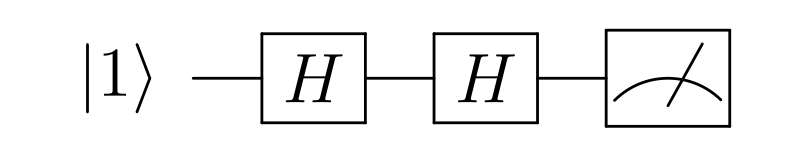
\includegraphics[width=0.8\linewidth]{Circuito1.png}
        \label{fig:placeholder}
    \end{figure}
    Questo esempio è molto semplice, ma per trasformazioni più complesse su più qubit diventerebbe difficile tracciare le operazioni. Nel prossimo circuito vediamo ad esempio un gate, $U$, che agisce su due qubit, un Hadamard sul primo qubit e una misurazione finale.
    \begin{figure}[H]
        \centering
        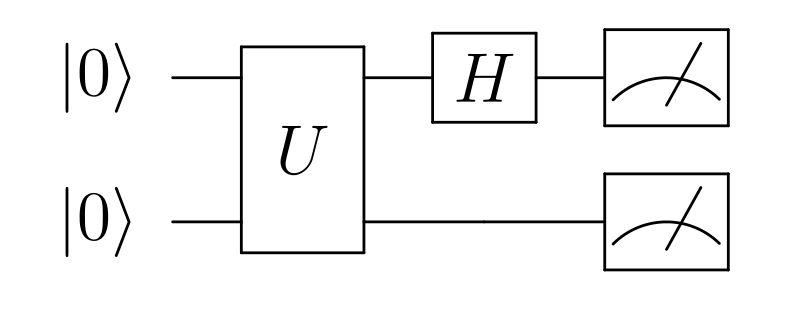
\includegraphics[width=0.8\linewidth]{Circuito2.png}
        \label{fig:placeholder}
    \end{figure}
    In alcuni casi inoltre è utile avere dei qubit extra per i risultati intermedi (tipicamente nello stato iniziale $\ket{0}$) chiamati \textbf{Ancilla Qubit}.
    \medskip
    \\ Un altro importante concetto è quello di \textbf{Gate controllati}. Tra questi gate vi è il CNOT visto precedentemente. In questa tipologia possiamo individuare un \textit{controllo} e un \textit{target}. Il controllo è rappresentato con un pallino pieno connesso da una linea ai qubit target.
    \\ Nel seguente circuito sono presenti 3 gate controllati: un Cnot, un generico operatore $U$ controllate e un secondo CNOT.
    \begin{figure}[H]
        \centering
        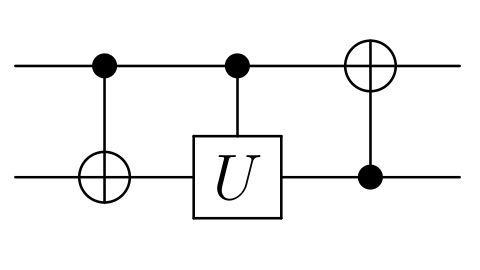
\includegraphics[width=0.7\linewidth]{Circuito 3.png}
        \label{fig:placeholder}
    \end{figure}
    Il controllo applica l'operazione al target se il qubit controllore si trova nello stato $\ket{1}$. Infine il controllo può andare vero entrambe le direzioni, sia verso l'alto che verso il basso.

    \begin{figure}[H]
        \centering
        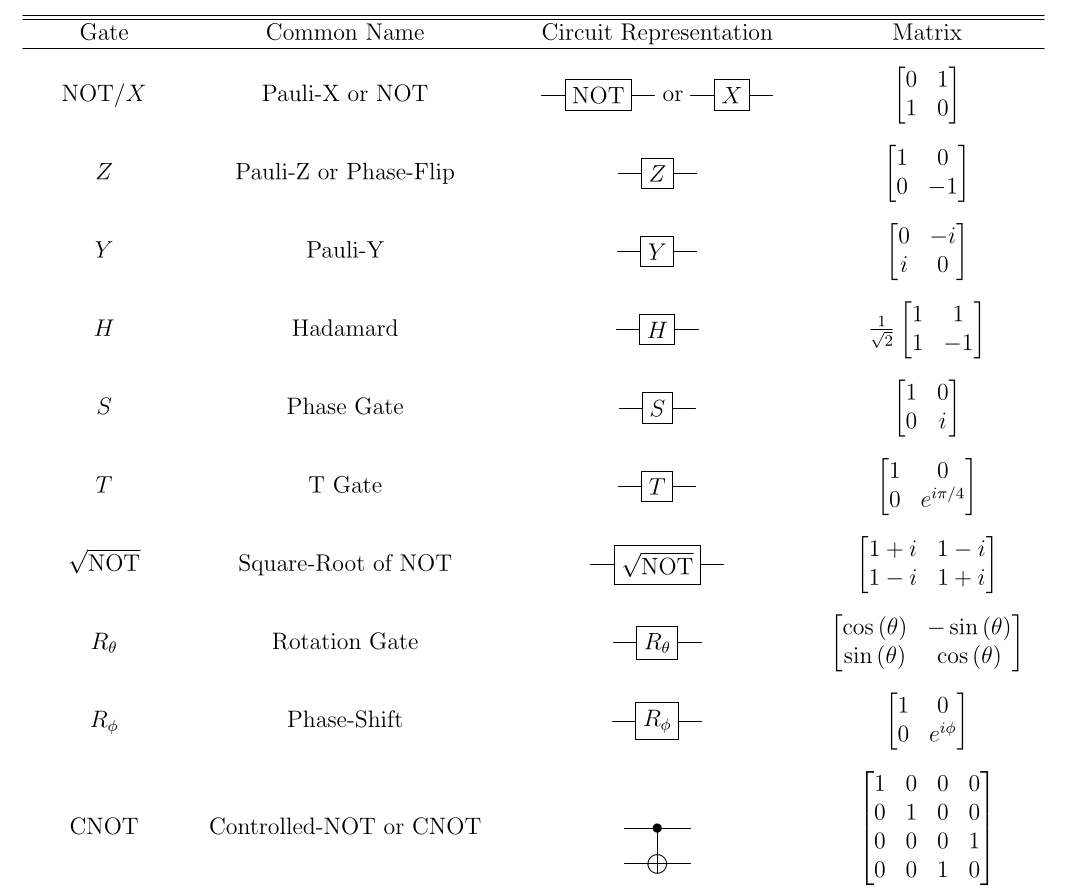
\includegraphics[width=1\linewidth]{gtable1.png}
        \label{fig:placeholder}
    \end{figure}
    \begin{figure}[H]
        \centering
        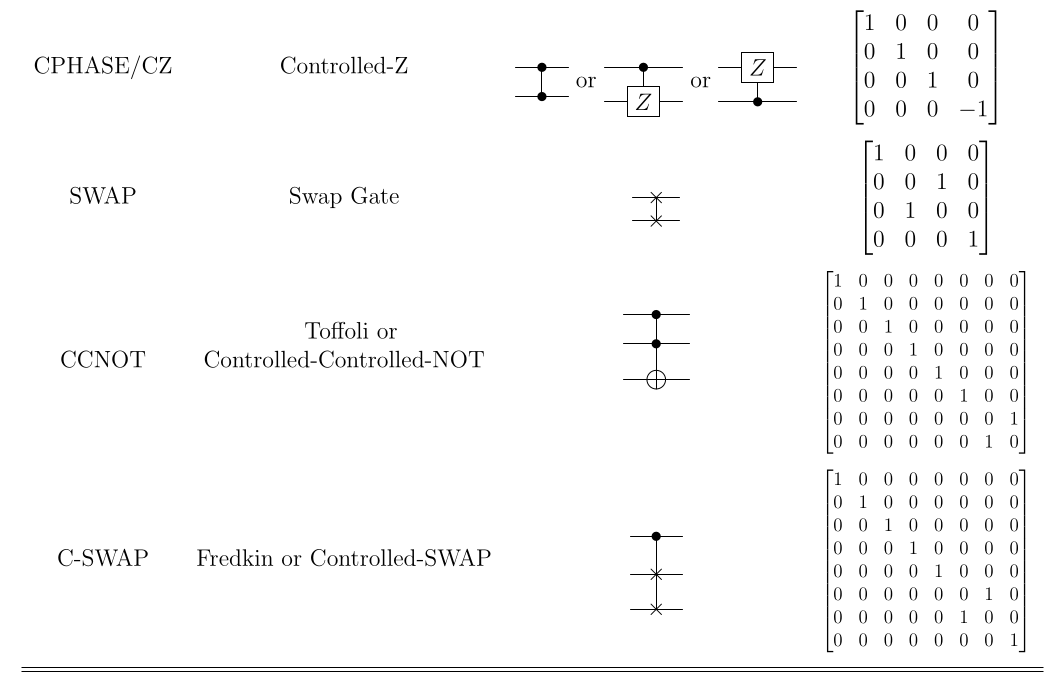
\includegraphics[width=1\linewidth]{gtable2.png}
        \label{fig:placeholder}
        \caption{Tabella dei Gate notevoli}
    \end{figure}

    \subsection{Effetto Zenone Quantistico}
    Ci sono alcuni meccanismi molto interessanti che avvengono nella meccanica di un qubit. Ipotizziamo di voler trasformare un qubit nello stato $\ket{0}$ nello stato $\ket{1}$ senza applicare trasformazioni unitarie.
    \\ Per qualche piccolo $\varepsilon$, possiamo misurare il qubit in una base ruotata dalla base $\{\ket{0},\ket{1}\}$ di un angolo $\varepsilon$. La probabilità di ottenere il qubit mosso di un angolo $\varepsilon$ cresce come $\varepsilon$ decresce. Definendo:
    \[
    \begin{split}
    \ket{v} = \cos(\varepsilon) \ket{0} + \sin(\varepsilon)\ket{1} \ \ \ 
    \\ \ket{w} = -\sin(\varepsilon)\ket{0} +\cos(\varepsilon)\ket{1}
    \end{split}
    \]
    \[
    \begin{split}
        P(\ket{v}) = |\braket{0|v}|^2 = |\cos(\varepsilon)|^2 \approx 1 - \varepsilon^2
        \\ P(\ket{w}) = |\braket{0|w}|^2 = |\sin(\varepsilon)|^2 \approx \varepsilon^2 \ \ \ \ 
    \end{split}
    \]
    Ripetendo il processo $\approx 1/\varepsilon$ volte, ruotando ogni volta la base di misurazione di $\varepsilon$, possiamo lentamente passare dallo stato $\ket{0}$ a $\ket{1}$.
    \\Qual'è la probabilità di ottenere un risultato diverso da quello desiderato? $1/\varepsilon \times \varepsilon^2 = \varepsilon$, quindi può essere arbitrariamente piccola. Questo è chiamato \textbf{Effetto Zenone Quantistico}, e uno dei suoi scopritori è stato \textit{Alan Turing}.
    \medskip
    \\ Una variante è il cosiddetto \textbf{Effetto della pentola osservata}. Stavolta vogliamo mantenere lo stato $\ket{0}$, ma il qubit tende a ruotare verso $\ket{1}$. Se continuiamo a misurare in base $\{\ket{0},\ket{1}\}$ ogni volta che il qubit ha subito una rotazione di un angolo $\varepsilon$, la probabilità che salti nello stato $\ket{1}$ è $\varepsilon^2$. Quindi ripetendo la misura $ \approx\frac{1}{\varepsilon}$ volte la probabilità di passare nello stato $\ket{1}$ è solo $ \approx \varepsilon$, nonostante la sua tendenza sicuro verso $\ket{1}$ senza la misurazione.

    \subsection{La Bomba di Elitzur-Vaidman}
    La \textbf{Bomba di Elitzur-Vaidman} è un altro interessante fenomeno quantistico scoperto negli anni '90.
    \\
    Facciamo finta di essere in un aeroporto quantistico in cui una valigia sospetta potrebbe contenere una bomba. Purtroppo l'idea di aprirla e controllare se dentro sia presente o meno un ordigno è fuori discussione poiché, nel primo caso, ne causeremmo la detonazione. Come fare?
    \\
    Supponiamo che la bomba sia progettata in modo da poter accettare una domanda posta con un bit classico, dove $b= 0$ significa che non abbiamo domandato, mentre $b=1$ significa che abbiamo posto la domanda. In questo caso abbiamo solo due possibilità: nella prima non abbiamo ottenuto alcuna informazione, mentre nella seconda rischiamo di far detonare la bomba se essa è veramente presente.
    \\
    Fortunatamente il nostro aeroporto è un sistema quantistico, quindi passiamo dal bit classico ad un qubit: $\ket{b} = \alpha\ket{0}+ \beta\ket{1}$. Ipotizziamo inoltre che in assenza di bomba lo stato $\ket{b}$ ci venga restituito. Se c'è una bomba, essa misura nella base $\{\ket{0},\ket{1}\}$. Se il risultato è $\ket{0}$ avremo come valore di ritorno $\ket{0}$, mentre se misura $\ket{1}$ la bomba esplode.
    \medskip
    \\
    Quello che possiamo fare è istanziare uno stato $\ket{0}$ e applicare una rotazione:
    \[
    R_\varepsilon =  \begin{bmatrix}
        \cos \varepsilon & -\sin \varepsilon \\
        \sin \varepsilon & \cos\varepsilon
    \end{bmatrix}
    \]
    Per cui lo stato diventa $\ket{b} = \cos(\varepsilon) \ket{0}+ \sin(\varepsilon)\ket{1}$. Se c'è la bomba, la probabilità che essa esploda al primo passaggio è $\sin^2(\varepsilon)\approx\varepsilon^2$, altrimenti otteniamo $\ket{0}$. Se non c'è nessuna bomba riotteniamo lo stato $\ket{b}$. 
    \\
    Ripetendo il processo, ogni volta che applichiamo $R_\varepsilon$, per $N = \frac{\pi}{2\varepsilon}$ volte, la probabilità totale di attivare la bomba, se essa è presente, è solo circa $N \sin^2(\varepsilon) \approx \frac{\pi}{2\varepsilon} \varepsilon^2 = \frac{\pi}{2} \varepsilon$. Misurando infine il nostro qubit per vedere se è $\ket{0}$ o $\ket{1}$, apprendiamo con certezza se la bomba c'è o no. Se la bomba è presente misuriamo lo stato $\ket{0}$, e se non è presente, la ripetuta applicazione di $R_\varepsilon$ ruota lo stato di $\frac{\pi}{2}$ e passiamo allo stato $\ket{1}$. Ovviamente l'esperimento non richiede solo un qubit, ma anche una bomba da interrogare quantisticamente!



    \section{Il problema della moneta, Distinguibilità, Stati a molti Qubit ed Entanglement}
    

        

    
\end{document}
